\section{Farm Model System}

No subsistema de quinta identificamos 3 processos nos quais o \"data flow\" pode sofrer ataques devido a vulnerabilidades.

\begin{figure}[h!]

	\centering

 	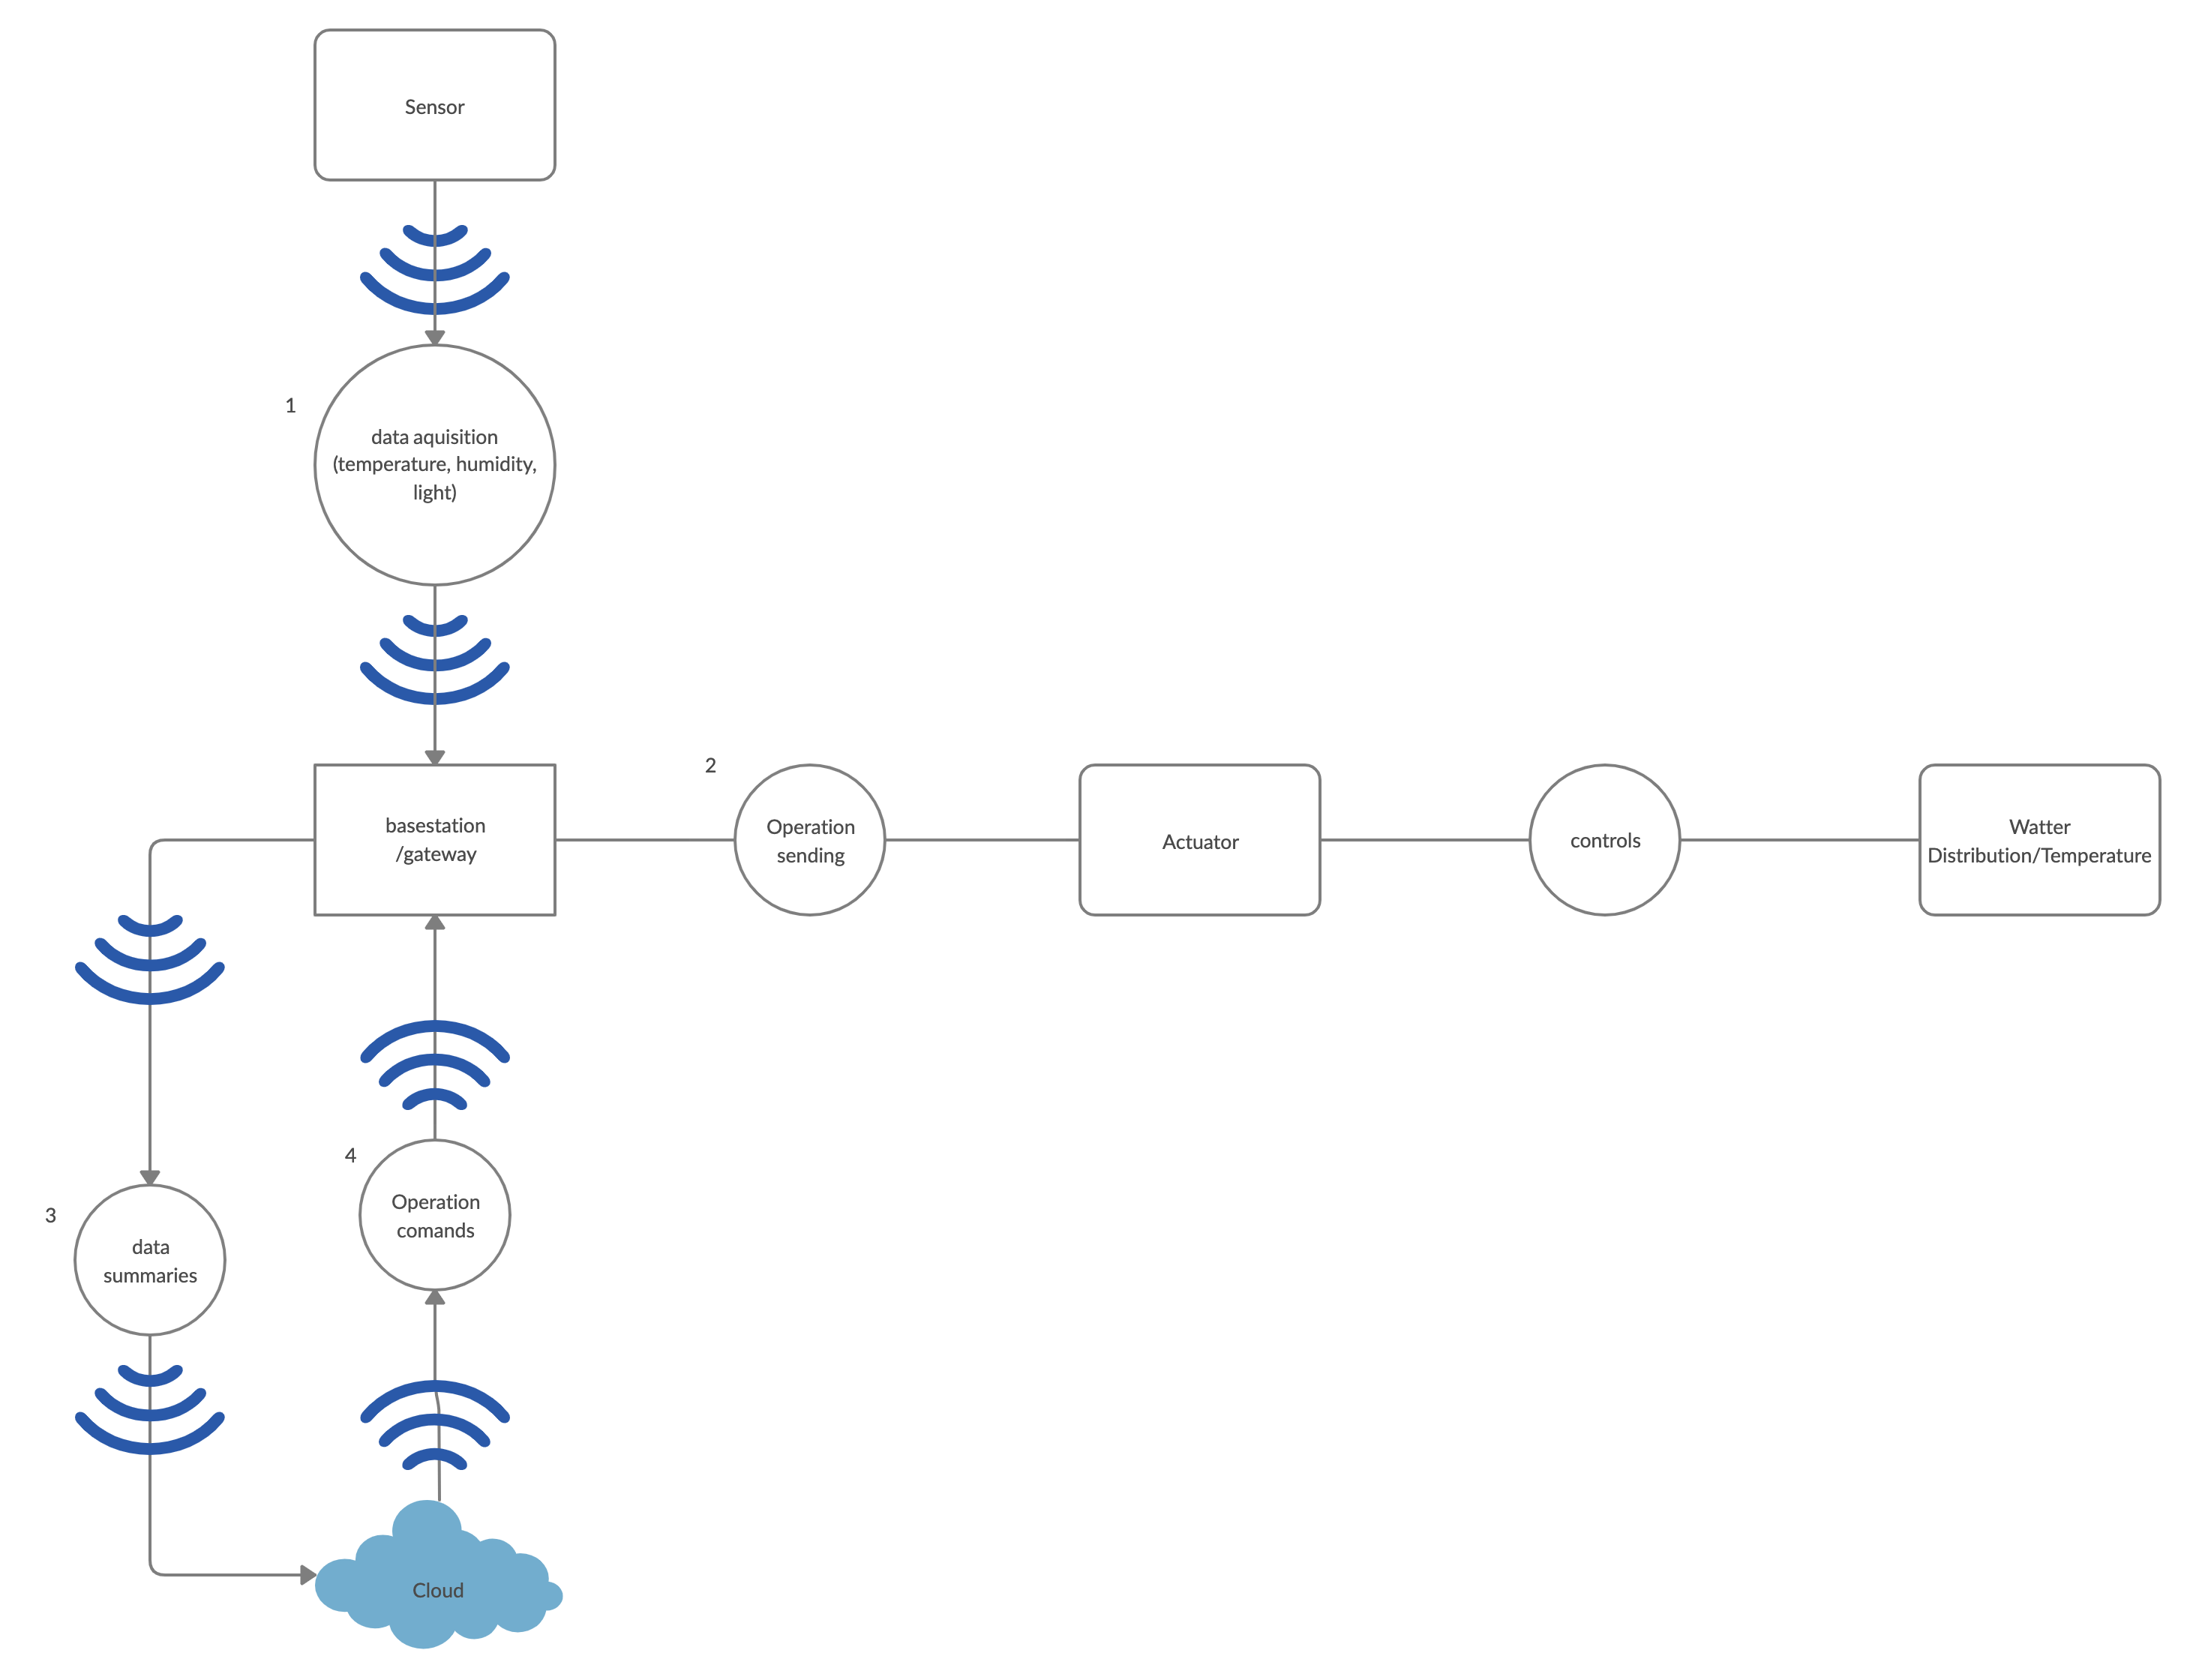
\includegraphics[scale = 0.15]{farmModel.png}

 	\caption {Model System for the Farm Subsystem}

  	\label {fig02}
\end{figure}

\subsection{1,3,4-Ataques de Spoofing}
\par\hfill
\par (1) Atacante pode fazer-se passar por um sensor e transmitir dados falsos.\newline
Correção => identificação de sensor.\newline

\par (3) Atacante pode fazer-se passar pelo gateway e transmitir dados falsos.\newline
Correção => identificação do gateway.\newline

\par (4) Atacante pode fazer-se passar pela cloud e transmitir dados falsos.\newline
Correção => identificação da cloud.\newline

\subsection{Ataques de Tampering}
\par\hfill
\par(Gateway) Um atacante pode alterar informação dos dados obtidos e apagar o log. \newline
Correção => ACLs devidamente feitas.\newline


\subsection{1,3,4-Ataques de Repudiation}
\par\hfill
\par(1)Atacante pode fazer-se passar por um sensor e enviar informação errada ao gateway.\newline
Correção => Identificação inequivoca de quem envia.\newline
\par(3)Atacante poe fazer-se passar pelo gateway e enviar informação errada para a cloud.\newline
Correção => Identificação inequivoca de quem envia.\newline
\par(4)Atacante pode fazer-se passar pela cloud e enviar informação errada para o gateway.\newline
Correção => Identificação inequivoca de quem envia.\newline

\subsection{1,3-Ataques de Information Disclosure}
\par\hfill
\par (1) Se a informação não for encriptada pode ser lida por um concorrente que não pague o serviço dispendioso e que possa obter vantagem competitiva.\newline
Correção => encriptação com chave simétrica conhecida apenas pelo sensor e  pelo gateway ou sistema de chave pública.\newline
\par (3) Se não for info encriptada pode ser lida pelo fornecedor da cloud que pode usar essa informação para um concorrente visando lucrar com a informação.\newline
Correção => encriptação com chave simétrica conhecida apenas pelo gateway e pelo front-end da aplicação.\newline

\subsection{1,3,4-Denial of Service}
\par\hfill
\par Um atacante pode tentar levar a cabo um ataque DoS nos processos 1 3 e 4.
Correção => No caso de tentative de Denial of Service podemos programar os nosso equipamentos para, após um x número de tentativas, bloquear o IP (temporáriamente) de quem está a gastar recursos do gateway sem se autenticar corretamente.\newline


\textit{Nota:} No caso da cloud, está a cargo do provedor do serviço tratar casos de tentativas de Denial of Service.\newline

\subsection{1,3,4-Elevation of privilege}
\par\hfill
\par (1) Verificar os dados recebidos como sendo dados comuns de um sensor.\newline
Correção => usar palavra chave simetrica ou assimetrica com não repúdio.\newline

\par (3) Verificar os dados recebidos como sendo dados comuns de um gateway.\newline
Correção => usar palavra chave assimetrica com não repúdio. \newline

\par (4) Verificar os dados recebidos como sendo dados comuns da cloud.\newline
Correção => usar palavra chave assimetrica com não repúdio. \newline



\textit{Nota:} Em relação ao 2º processo, como a ligação é feita usualmente por cabo não existem problemas muito serios, apenas ataques fisicos devem ser considerados, como cortar os cabos de ligação para impedir o funcionamento do sistema.\newline


\section{Considerações Finais}

\subsection{Sensores}
\par\hfill
\par Como visto anteriormente os sensores devem ser autenticado inequivicamente e enviar a informação recolhida encriptada para garantir a veracidade e origem dos dados.\newline
\par Para garantir que um atacante não adiciona um sensor com código modificado de forma a de alguma forma comprometer o sistema, os sensores a poderem comunicar com o gateway devem ser definidos á partida.\newline

\subsubsection{ZigBee sensors}
\par\hfill
\par Quanto a identificação dos mesmos esta é feita de forma inequivoca, garantindo que não é possível um atacante replicar o id do sensor.\newline 
Usa AES-128 encryption para garantir a encriptação dos dados.

\subsubsection{TelosB motes}
\par\hfill
\par Usa TinyOS como a biblioteca criptográfica normalmente, esta tem um algoritmo eficiente com overhead de encriptação na ordem dos microsegundos, garantindo a integridade do sistema de forma rápida e utilizando poucos recursos.\newline
\par Relativamente barato.

\subsubsection{Arduino}
\par\hfill
\par Usa AES-128 encryption para garantir a encriptação dos dados.\newline
\par Usa X.509 que é um padrão ITU-T para infraestruturas de chaves públicas (ICP),permitindo autenticação forte.
\par Permite programar os processos de autenticação dos sensores e como estes comunicam. 

\subsubsection{Raspberry}
\par\hfill
\par Usa mecanismos de chave pública para garantir a encriptação.
\par Relativamente barato.\newline


\par Concluindo, se o foco for ter uma encriptação o mais forte possível, devemos optar por utilizar um raspberry sensor visto este usar mecanismos de chave pública. No entanto estes pesam no requisito de transmissão de dados de forma mais rápida possível. O TelosB motes tem essa vantagem embora não possua uma encriptação tão boa como os restantes sensores.\newline


\textit{Nota:} Se se pretende uma tecnologia de encriptação que se mantenha segura sem ser necessário mudá-la, o AES-128 não é aconselhado visto que já está em fase de se tornar deprecated (estima-se que por volta de 2030) e a quinta supõe-se que deva permanecer em funcionamento por mais de 10/11 anos aquando da redação deste relatório.\newline



\subsection{Gateway}
\par\hfill
\par No caso da informação que flui do gateway para a cloud é preciso garantir que estamos a enviar dados encriptados visto que o provedor da cloud pode utilizar os dados que registamos para proveito próprio, ou até mesmo um terceiro que comprometa a segurança da cloud não possa tirar proveito da nossa informação. Desta forma temos de garantir que apenas o nosso gateway e a aplicação no lado do cliente tenha acesso á chave de encriptação e desencriptação. Note-se que se deve fazer uso de encriptação forte para garantir de forma mais consistente a segurança dos dados.\newline

\subsection{Cloud}
\par\hfill
\par O tratamento da segurança da informação na cloud (encriptada ou não) é responsabilidade do provedor do serviço, logo este relatório não englobará medidas para proteger a cloud de qualquer ataque. Apenas de proteger a informação que lhe é passada encriptando-a.\newline
Para além disso é necessário ainda assim que tenhamos uma forma inequivoca de garantir o não repúdio por parte do gateway face a cloud e vice-versa, nesta matéria aconselha-se o uso de um certificado digital.\newline 
